\documentclass[11pt,a4paper]{article}

\usepackage{url}
\usepackage{graphicx}
\title{Establishing Network connection and SSH connection}
\author{e-Yantra Team}
\date{\today}

\begin{document}
	\maketitle
	\newpage
	\tableofcontents
	\newpage
	\section{Tutorial Name}
	\textbf{Objective:} In this tutorial we will learn how to establish a network connection in an R-Pi. We shall also learn how to connect a remote PC with a Raspberry Pi using SSH connection.
	\section{Prerequisites}
	One should be aware of :
	\begin{itemize}
		\item Various commands that are used in LXterminal.
		\item How to connect to Wireless network
	\end{itemize}
	
	\section{Hardware Requirement}
	\begin{enumerate}
		\item Raspberry Pi (I will be using Version 2 Model B)
		\item Monitor
		\item HDMI cable
		\item Keyboard
		\item Mouse
		\item Wireless adapter
		\item Power adapter
		\item PC(either Windows or Linux)
	\end{enumerate}
		
	\section{Software Requirement}
	MobaXterm(for Windows user)
	
	\newpage
	\section{Theory and Description}
	Secure Shell, or SSH, is a cryptographic (encrypted) network protocol for initiating text-based shell sessions[clarification needed] on remote machines in a secure way.
	
	This allows a user to run commands on a machine's command prompt without them being physically present near the machine. It also allows a user to establish a secure channel over an insecure network in a client-server architecture, connecting an SSH client application with an SSH server.Common applications include remote command-line login and remote command execution, but any network service can be secured with SSH. The protocol specification distinguishes between two major versions, referred to as SSH-1 and SSH-2.
	
	SSH was designed as a replacement for Telnet and other insecure remote shell protocols such as the Berkeley rsh and rexec protocols, which send information, notably passwords, in plaintext, rendering them susceptible to interception and disclosure using packet analysis.
	\begin{figure}[h!]
		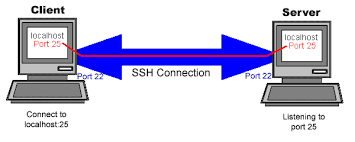
\includegraphics{ssh.png}
		\centering
	\end{figure} 
	
	\textbf{Applications of SSH or OpenSSH protocol}
	\begin{itemize}
		\item For login to a shell on a remote host (replacing Telnet and rlogin)
		\item For executing a single command on a remote host (replacing rsh)
		\item For setting up automatic (passwordless) login to a remote server (for example, using OpenSSH)
		\item Secure file transfer
		\item In combination with rsync to back up, copy and mirror files efficiently and securely
		\item For forwarding or tunneling a port (not to be confused with a VPN, which routes packets between different networks, or bridges two broadcast domains into one).
		\item For using as a full-fledged encrypted VPN. Note that only OpenSSH server and client supports this feature.
		\item For forwarding X from a remote host (possible through multiple intermediate hosts)
		\item For browsing the web through an encrypted proxy connection with SSH clients that support the SOCKS protocol.
		\item For securely mounting a directory on a remote server as a filesystem on a local computer using SSHFS.
		\item For automated remote monitoring and management of servers through one or more of the mechanisms discussed above.
		\item For development on a mobile or embedded device that supports SSH.
	\end{itemize}
	
	\newpage
	\section{Experiment}
	In order to use a Raspberry Pi remotely we need to configure its wireless settings as follows:
	\begin{enumerate}
		\item Insert the SD card (with Raspbian OS already written) into the micro SD slot in an R-Pi.
		\item Connect the wireless adapter, keyboard , mouse and monitor (using a HDMI cable) to the Raspberry Pi.
		\item Power on the board and monitor.You will notice a set of code running on the monitor.
		\item Enter the set user name and password and then type 'startx' command to launch the GUI.
		\begin{figure}[h!]
			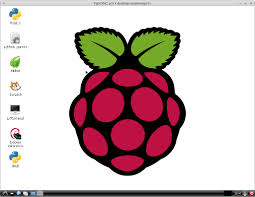
\includegraphics[width=10cm,height=8cm]{r1.jpg}
			\centering
		\end{figure} 
		\item Click on the icon at the bottom-left on the screen. This is the start icon.
		\item Select LXTerminal option. A terminal window opens.
		\newpage
		\begin{figure}[h!]
			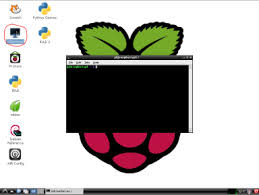
\includegraphics[width=10cm,height=8cm]{lxt.jpg}
			\centering
		\end{figure}
		\item  Some of the previous versions of Raspbian OS do not support wireless module. To know about the version you are using type "uname -a". To upgrade to the latest one type "sudo apt-get upgrade".
		\item Connect your wireless adapter . To check if its connected type "lsusb"(We used D-link adapter which is highlighted in yellow) 
		\begin{figure}[h!]
			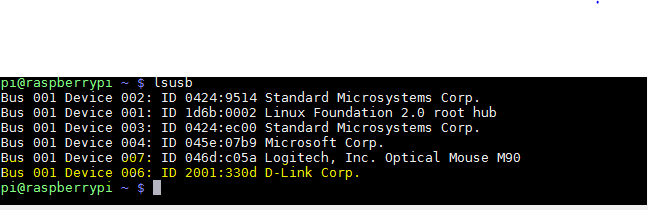
\includegraphics{Lsusb.PNG}
			\centering
		\end{figure}
		\newpage
		\item Now type "sudo nano /etc/network/interfaces" and press enter. You will see the following window:
		\begin{figure}[h!]
			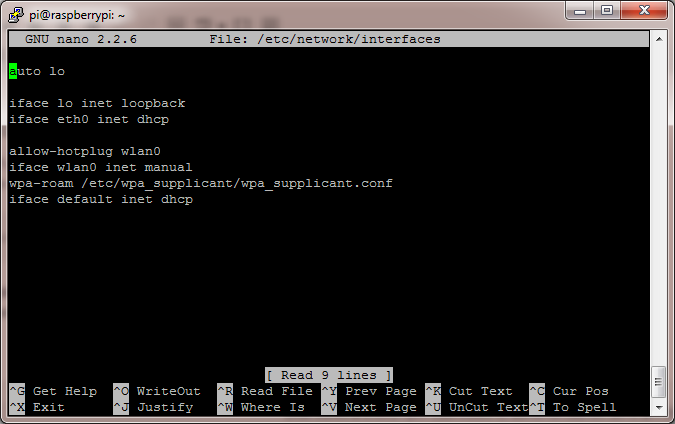
\includegraphics[width=10cm,height=8cm]{iwifi.png}
			\centering
		\end{figure}
		\item Change the code by adding the following lines:
		\begin{figure}[h!]
			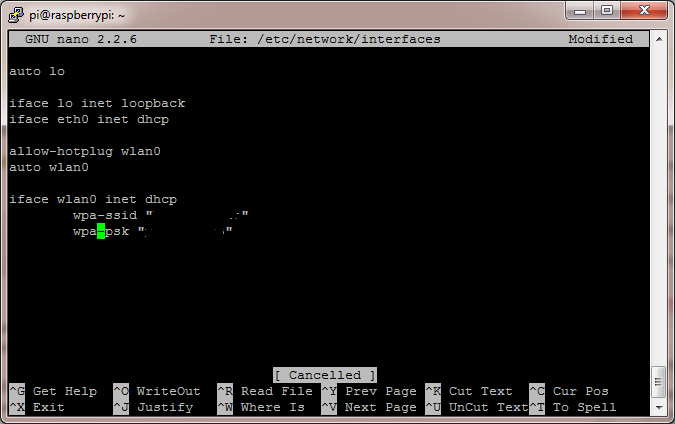
\includegraphics[width=10cm,height=8cm]{wificon.png}
			\centering
		\end{figure}
		\item Add in the SSID(username) and Password of your wifi. Then for changes to take effect type "sudo /etc/init.d/networking restart" 
		\item Type "ifconfig" to obtain the IP address of R-Pi etc. It will be under wlan0(written as inet address).
	\end{enumerate}
	
		
	To start using the Raspberry Pi remotely follow these steps:
	\begin{enumerate}
		\item A windows user should download MobaXterm (latest version) using the following link: \url{http://mobaxterm.mobatek.net/}
		\item Run the .exe file and open the application.
		\begin{figure}[h!]
			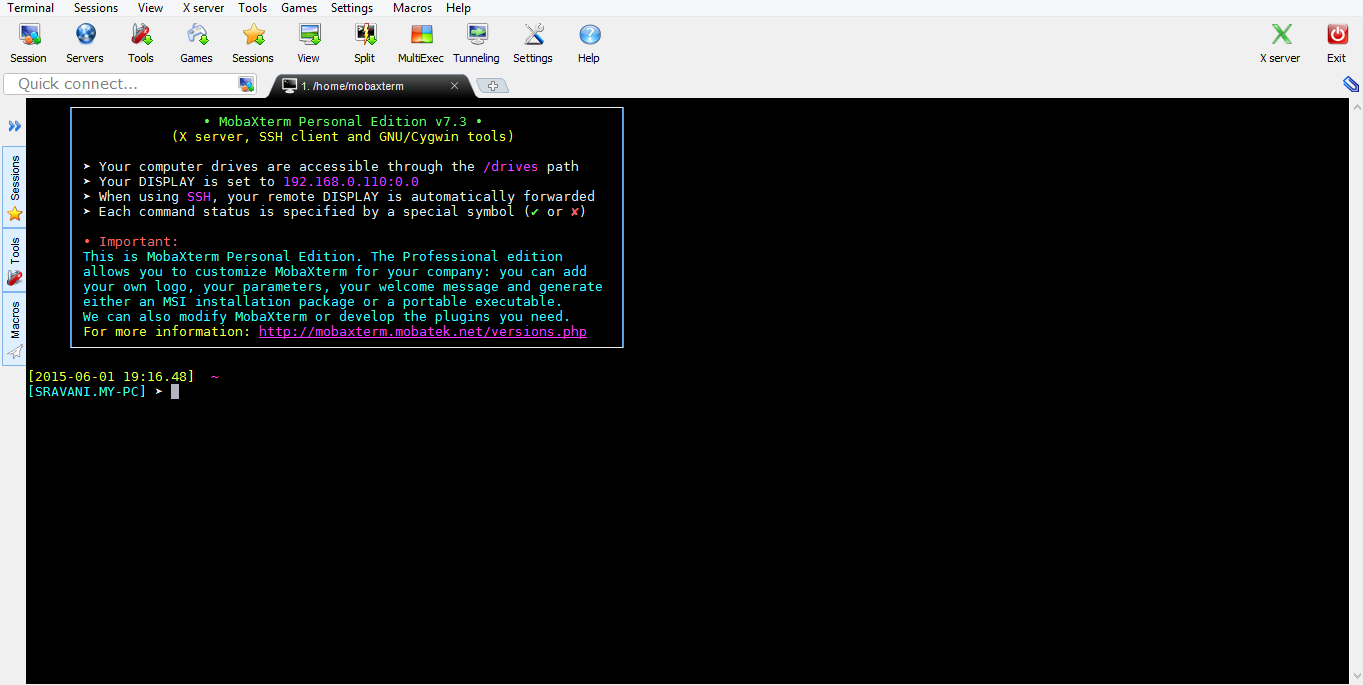
\includegraphics[width=10cm,height=6cm]{M1.PNG}
			\centering
		\end{figure}
		\item Then select the session option on the toolbar.
		\begin{figure}[h!]
			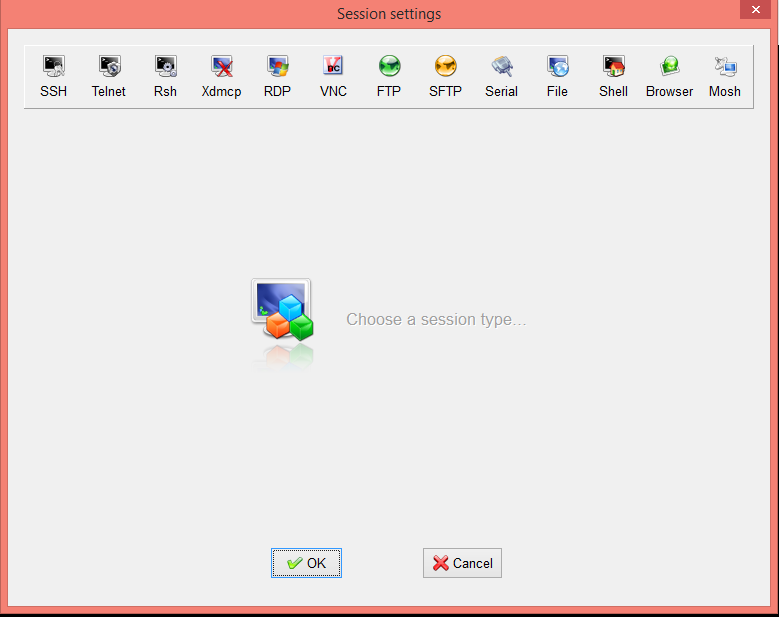
\includegraphics[width=10cm,height=8cm]{M2.PNG}
			\centering
		\end{figure}
		\newpage
		\item Click on the SSH option. A settings window opens as shown
		\begin{figure}[h!]
			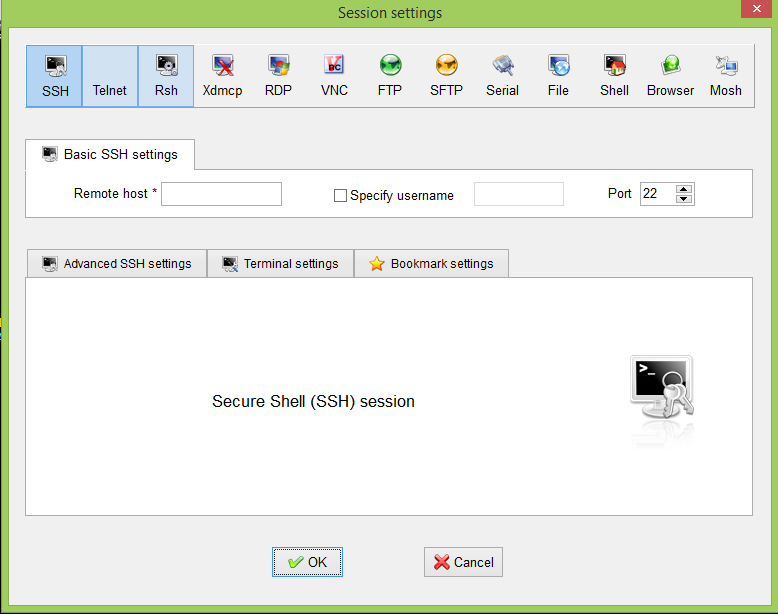
\includegraphics[width=6cm,height=5cm]{M3.PNG}
			\centering
		\end{figure}
		\item Enter the IP address of the R-pi in the Remote host field and in the 'Advanced SSH settings' option configure the remote environment either as 'Interactive shell (terminal based)' or as an 'LXDE desktop(GUI based)'and click OK
		\item If you are using the Interactive shell environment login to the R-Pi using the following command: ssh -X pi@192.168.0.4 (IP address of pi) and then enter the login id and password to start using the Pi remotely.
		\item If you are using the LXDE desktop i.e. the GUI environment then use LX terminal icon to start programming the Pi.
		\begin{figure}[h]
			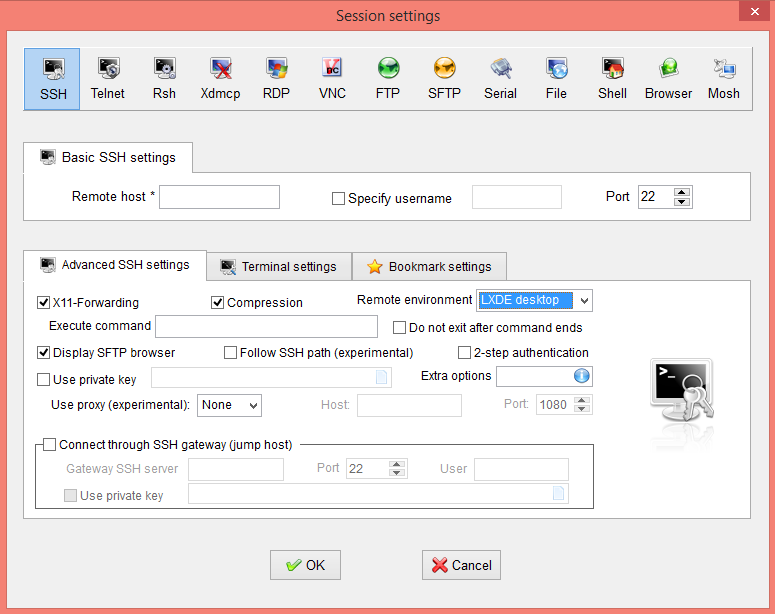
\includegraphics[width=10cm,height=6cm]{M4.PNG}
			\centering
		\end{figure}
		\newpage
		\item Also the established session is saved. So the next time you want to access directly click on the R-Pi's address mentioned in the saved session option to start using the Pi remotely.
		\begin{figure}[h!]
			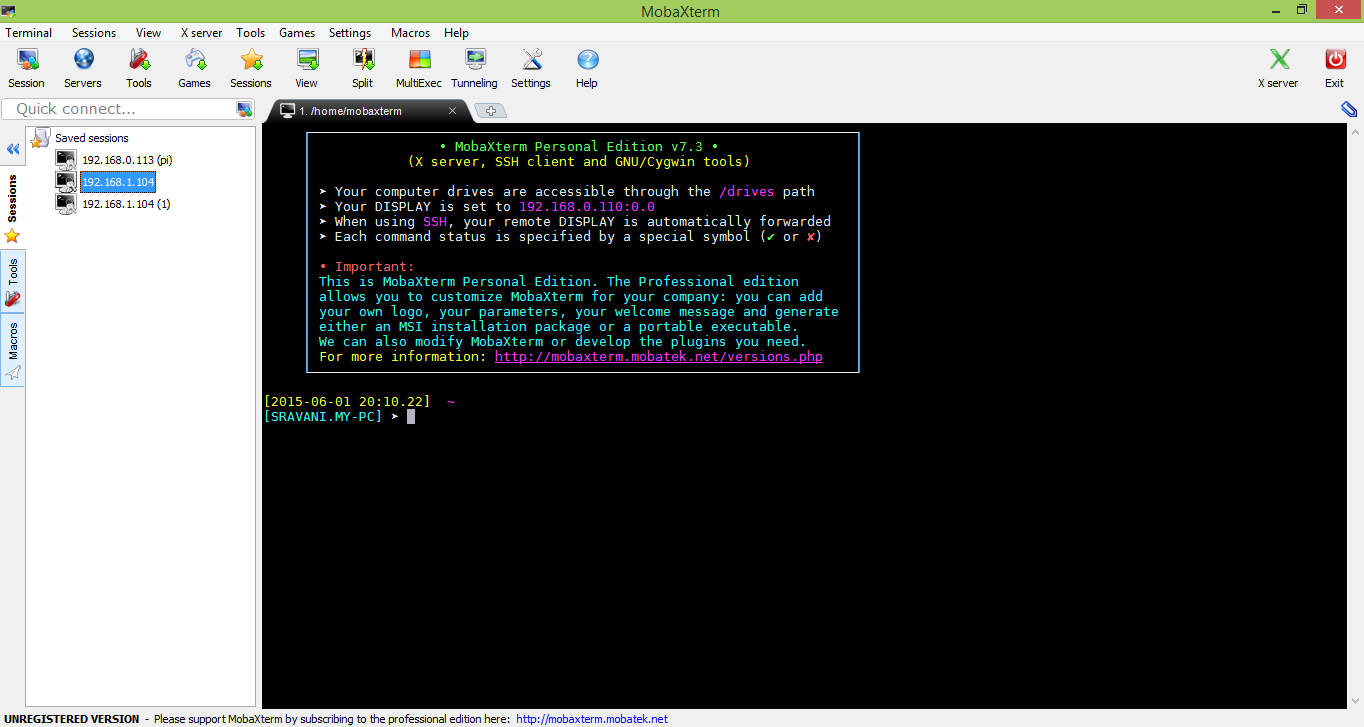
\includegraphics[width=10cm]{M5.PNG}
			\centering
		\end{figure}
	\end{enumerate}

	\textbf{Note:} A linux user needn't download any Xterm file. They can directly start accessing the R-Pi using the command: ssh -X pi@192.168.0.4 (IP address of pi) and then entering the login id and password for using the Pi remotely.
	
	\section{References}
	\begin{itemize}
		\item \url{http://en.wikipedia.org/wiki/Secure_Shell}
	\end{itemize}
\end{document}



